% Created 2010-11-07 Sun 20:24
\documentclass[11pt]{article}
\usepackage[utf8]{inputenc}
\usepackage[T1]{fontenc}
\usepackage{fixltx2e}
\usepackage{graphicx}
\usepackage{longtable}
\usepackage{float}
\usepackage{wrapfig}
\usepackage{soul}
\usepackage{t1enc}
\usepackage{textcomp}
\usepackage{marvosym}
\usepackage{wasysym}
\usepackage{latexsym}
\usepackage{amssymb}
\usepackage{hyperref}
\tolerance=1000
\providecommand{\alert}[1]{\textbf{#1}}

\title{AS-0.3301 Project Plan: Tower Defense}
\author{Joel Pitkänen <joel.pitkanen@tkk.fi> (82156A),\\ Joonas Nissinen <joonas.nissinen@tkk.fi> (84362C),\\ Ilari T. Nieminen <ilari.nieminen@tkk.fi> (60628W)}
\date{08 November 2010}

\graphicspath{{figures/}}

\begin{document}

\maketitle

\setcounter{tocdepth}{3}
\tableofcontents
\vspace*{1cm}

\section{Introduction}
\label{sec-1}


This document is a project plan for a tower defense game, to be
developed during the fall of 2010 for the course AS-0.3301 (C++
programming). The following sections describe the high-level features
and the approximate architecture of the game. 
\section{Specification of requirements}
\label{sec-2}


This section describes the basic features that the game will have
(core features) as well as features that will be added if there is
enough time (additional features).
\subsection{Core features}
\label{sec-2_1}


   The game will fulfill the minimum requirements as specified in the
   project description as well as some additional requirements:

\begin{itemize}
\item Mouse input with keyboard shortcuts
\item Multiple enemy types with different properties (hit points, speed)
\item Multiple upgradeable tower types: direct, splash and special damage
\item Easy-to-read, easy-to-edit format for maps
\item Towers can be placed at any time
\item Dynamic paths for enemies
\item Multiple terrain types
\item Player profiles, player progress
\end{itemize}
\subsection{Additional features}
\label{sec-2_2}


   A subset of these features will be implemented, depending on how
   much time the core features will take.

\begin{itemize}
\item Multiple entry and exit points for enemies
\item Fast-forward: When nothing interesting is happening, the player
    may speed up the game
\item Checkpoints: Player may return to a checkpoint instead of having
    to start the level over in case of seriously suboptimal tower
    placement.
\item Different firing strategies for towers: Sort the enemies by
    several properties: shortest remaining path to goal, speed, hit
    points, maximum hit points.
\item Tower statistics: See how much damage each tower has inflicted
\item Scrollable maps
\item Graphical map editor
\end{itemize}
\section{Program architecture}
\label{sec-3}

This section describes the overall structure of the game.

\subsection{Class structure}

The class structure is shown in Figure \ref{fig:classdiagram}.

\label{sec-3_2}
\subsubsection*{Map}
\label{sec-3_2_1}

    Methods for reading (and writing?) maps, keeps track of towers and waves of enemies. 
\subsubsection*{Tower}
\label{sec-3_2_2}

    Virtual base class for towers
\subsubsection*{Projectile}
\label{sec-3_2_3}

    Visible graphical ammunition for some towers
\subsubsection*{Mob}
\label{sec-3_2_4}

    Virtual base class for mobs
\subsubsection*{Timer}
\label{sec-3_2_5}

    For handling game time / real time (predictable passage of time inside the game)    
\subsubsection*{Player}
\label{sec-3_2_6}

    Player profile stores the progress and settings
\subsubsection*{GameState}
\label{sec-3_2_7}

    Base class for gamestates. A gamestate is essentially one screen
    of the game (e.g. MainMenuState, GameplayState)
\subsubsection*{GameStateManager}
\label{sec-3_2_8}

    Manages a LIFO stack of gamestates.  Updates the topmost state on
    the stack.
\subsubsection*{Renderer}
\label{sec-3_2_9}

    Draws the map and everything contained in it (towers, mobs etc.)
\subsubsection*{Camera}
\label{sec-3_2_10}

    A movable camera. Used by the renderer to draw objects relative to camera coordinates.

\begin{figure}[h!]
\centering
  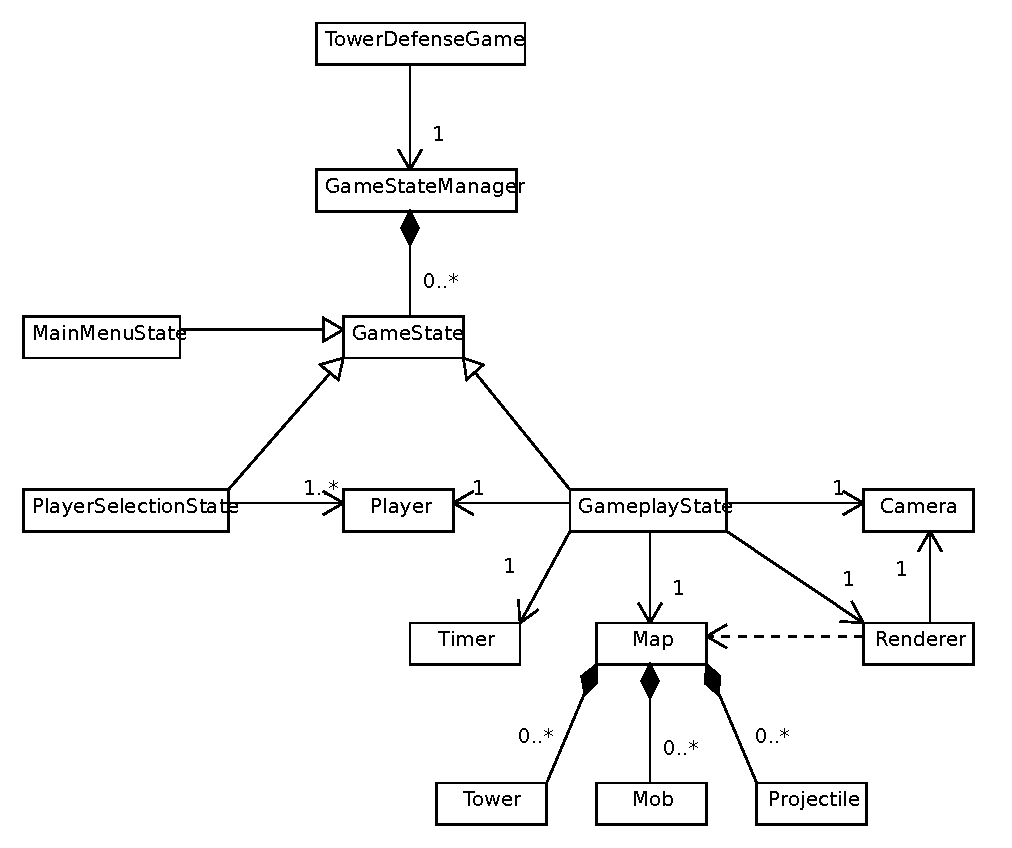
\includegraphics[width=0.9\textwidth]{diagram.pdf}
  \caption{An overview of the relations of the classes}
\label{fig:classdiagram}
\end{figure}

\subsection{Data structures and algorithms}
\label{sec-3_1}

A priority queue to keep track of game events (arrival of enemies,
damage to enemies)

The map will have an associated graph, which will be used to determine
the shortest path to the goal for enemies using a shortest-path
algorithm such as Dijkstra's algorithm.

\subsection{Persistence and file formats}
\label{sec-3_3}

Settings and player progress will be stored in an SQLite database.

The maps will be stored in an easy-to-edit format in text files, at
least unless a graphical map editor will be implemented. 
\subsection{Possible problems}
\label{sec-3_4}


  If the number of enemies on the map is large, one possible
  bottleneck is the dynamic path calculation, which would be done for
  all enemies at the same time (whenever the player places a tower
  that might interfere with their route); this could cause a
  noticeable slowdown. The path-finding could be placed in a separate
  thread to allow faster processing whenever multiple cores or
  processors are available, or the time allotted to path-updating
  could be limited in some fashion. Also, the target selection for
  towers must be implemented in a sane way, so that only a subset of
  enemies are considered as possible targets.

  The role of projectiles is not yet completely determined. For damage
  calculation, it would be easiest to determine the time of the hit
  when the projectile is fired and then just update the location of
  the projectile to match the reality. If projectiles are allowed to
  miss, the situation becomes a bit more complex, as the aiming has to
  be done in a smart manner at least if some projectiles are slow.

\section{Task sharing}
\label{sec-4}

Discussion over implementation issues during coding will be mostly
done over IRC. Coding sessions for the whole group will be organized
if personal schedules allow.

The rough division of tasks is as follows:

\begin{itemize}
\item Joel: User interface, graphics
\item Joonas: Graphics, game data systems
\item Ilari: Game logic
\end{itemize}
\section{Testing}
\label{sec-5}

Automated unit tests will be made for individual parts of the
program. These will especially help in making sure that the corner
cases are handled correctly. Making sure that individual parts of the
program work before proceeding saves time from future tests as you
have less lines of code to check for possible errors. Features will be
tested in practice after their implementation to make sure that they
function as planned.

Certain parts of the program require special attention with testing.
For example the map file reading has to be tested rigorously, as users
can provide arbitrary files to the program and so it must be able to
handle any input gracefully.

As all the individual pieces start to merge together and we have at
least a playable prototype, manual testing of different situations in
the working program has to be applied.

When the game is nearly finished, we will try to recruit a monkey who
wants to test it. The monkey will run as many different scenarios as
possible.

\section{Schedule}
\label{sec-6}

This section describes the planned weekly schedule for the project.

\subsection*{Week 45}

During this week, the program structure and the interfaces will be
specified in more detail, making it possible to do more individual
work. Implementation starts.

\begin{center}
\begin{tabular}{rrp{0.7\textwidth}}
\hline
Person  & Time (h) & Notes \\
\hline
Joel & 12 & Planning, implementation for the gamestate system.\\ 
Joonas & 10 & Planning, implementation for the map reading system.\\
Ilari & 10 & Planning, header files related to game.
\end{tabular}
\end{center}

\subsection*{Week 46}

On this week, we will have a first ``playable'' (there is something to
point and click) protype, making sure that the specifications from the
previous week are enough to allow efficient implementation of features
for each team member.

\begin{center}
\begin{tabular}{rrp{0.7\textwidth}}
\hline
Person  & Time (h) & Notes \\
\hline
Joel & 15 & Implementation for Camera and Renderer. Initial implementation for the UI\\ 
Joonas & 15 & Implementation for the player database system. Starting with the graphics.\\
Ilari & 16 & Initial tower and enemy implementation, implementation of pathfinding and tower operation.
\end{tabular}
\end{center}

\subsection*{Week 47}

Core features will be finalized during this week. The result should be
a reasonably working game which satisfies the minimum requirements
specified in section \ref{sec-2_1}. The implementation of additional
features commences.

\begin{center}
\begin{tabular}{rrp{0.7\textwidth}}
\hline
Person  & Time (h) & Notes \\
\hline
Joel & 15 & Finalizing the UI\\
Joonas & 14 & Finalizing the graphics. Helping with other stuff.\\
Ilari & 14 & Implementation of the rest tower and enemy types. Writing the rest of game ``rules''.
\end{tabular}
\end{center}

\subsection*{Week 48}

Testing of the whole game, implementation of additional features. The
report will be written.

\begin{center}
\begin{tabular}{rrp{0.7\textwidth}}
\hline
Person  & Time (h) & Notes \\
\hline
Joel & 15 & Documentation and testing\\
Joonas & 15 & Additional features, documentation and testing.\\
Ilari & 14 & Documentation
\end{tabular}
\end{center}

\subsection*{Week 49}

The demo week. Final bug fixes, aesthetic changes.

\begin{center}
\begin{tabular}{rrp{0.7\textwidth}}
\hline
Person  & Time (h) & Notes \\
\hline
Joel & 8 & Polishing\\
Joonas & 8 & Finalizing what's left, finishing up the additional features and documentation.\\
Ilari & 8 & Testing, improving playability
\end{tabular}
\end{center}

\subsection*{Summary}

The total time planned for the project is approximately 60 hours per
person. This time does not include the time planning the project
before week 45.

\section{External libraries}
\label{sec-7}


We will use ClanLib, as it provides many useful features for a game:
high-level rendering, collision detection, sprites, etc. The Boost
libraries can also provide useful tools for many parts of the project,
for example Boost Test Library can be used to aid in the testing and
Boost Graph Library can be used to help with the dynamic path
generation for enemies.



\appendix
\clearpage
\section{GUI Sketch}

\begin{figure}[h]
  \centering
  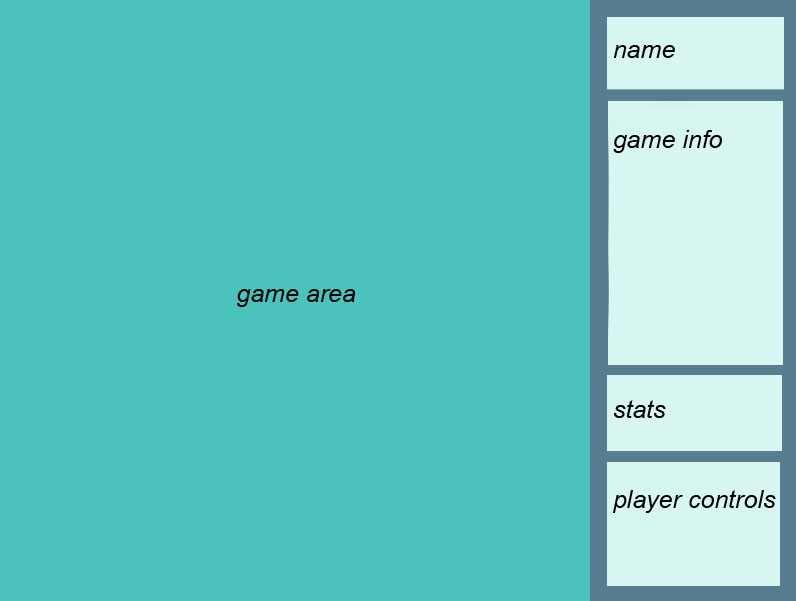
\includegraphics[width=0.8\textwidth]{sketch.png}
  \caption{An initial plan for the organization of the graphical user
    interface}
\end{figure}

\clearpage
\section{Map file format}

A draft for the map file format.

\begin{verbatim}
!MAP
LEVEL 1: Level name
	#########################
	#SSSSSSSSSSSSSSSSSSSSSSS#
	#SSSSSSSSSSSSSSGGGGGGSSS#
	#SSSSS          GGGGGGGS#
	#SR     E       GGGGGSSS#
	#SR             GGGGGSSS#
	#SR     GRS          RSS#
	#SR                  RSS#
	#SSSGGGGGGSSWW       RSS#
	2                    RSS#
	#RRRRRSSGGGS         RRR#
	1                   RRRR#
	#########################
WAVES:
	1: 6 enemy_type_1
	2: 4 enemy_type_1, 5 enemy_type_2
	3: 6 enemy_type_2, 5 enemy_type_3
					.
					.
					.
	n: 1 enemy_type_x, 2 enemy_type_y
\end{verbatim}

Map files store the data responsible of level information, i.e. the
actual map in ASCII format and the information about the enemy
waves. The file always starts with exactly same arbitrary text,
``!MAP'', which can be used to identify the file as a map file.

Immediately after the identification follows the level information
starting with the level number, name and the map layout. The playable area
of the map is the area enclosed within the \#-characters. Characters
like S,R,G and W represent different types of grounds on which you the
player can build certain types of towers. Empty characters represent
the space in which the enemies can walk in towards their goal, which
the letter E is representing in the example. There are also ground
types on which the enemies can traverse but can be also built upon by
the player. Numbers 1 and 2 in this case represent the entry points
for the enemies.

After the map layout comes the information about the waves of
enemies. The lines always start with the wave number. After the wave
number comes the information of the number of enemies and their
type. Different types are separated by a comma. For a variable delays
between waves or enemies, some additional information needs to be
added.

The information could be stored in a more condensed manner, however it
would be nice if the format is logical for the untrained human eye as
well. Depending on the features that the maps will be required to
have, some human readability might be lost during the project.

\end{document}
